\documentclass[../main.tex]{subfiles}

\begin{document}

This chapter provides an introduction to clinical trials and their importance to biomedical research. Section 2.1 provides background for and discusses the motivation and reasoning in focusing on clinical trials. Section 2.2 examines challenges in trial recruitment. Section 2.3 discusses past work in patient matching for clinical trials using electronic software. Section 2.4 examines challenges in electronic screening for trials using NLP. Section 2.5 discusses research in NLP methods for clinical trial recruitment, while Sections 2.6 and 2.7 examine published corpora related to clinical trials and clinical knowledge bases. Section 2.8 provides a summary of the chapter.

\section{The Importance of Clinical Trials}

A clinical trial is a prospective study comparing the effects and value of an intervention (typically a medication, biologic, or procedure) against a control group without it \cite{friedman2015fundamentals}. Clinical trials are considered "controlled" when a control group not receiving an interventional treatment is used for comparison, and "randomized" when participants are randomly placed in said treatment or control groups. Randomization is considered ideal for reducing risk of investigator bias and producing study groups closely in proportion to known risk factors. Randomized controlled trials (RCTs) are widely recognized as the best available method to determine if a given intervention is safe and effective \cite{friedman2015fundamentals}.

Eligibility for a clinical trial is determined by a trial's \textit{eligibility criteria}, which are free-text descriptions of required conditions, treatments, laboratory tests and so on. Eligibility criteria are composed of \textit{inclusions}, which patients \textit{must meet}, and \textit{exclusions}, which patients \textit{must not meet} in order to be eligible. The extent to which trial results can be assumed to be generalizable to patients not participating in a trial but with comparable health status is determined by \textit{external validity} \cite{rothwell2005external}. External validity can be influenced by a number of factors, first and foremost the selection of patients potentially eligible for a trial. Finding patients appropriately meeting eligibility criteria in as unbiased way as possible is thus critical to drawing meaningful conclusions from clinical trials, and ultimately scientific progress and improvement of human health.

\section{Challenges in Recruitment for Clinical Trials}

Many clinical trials fail to meet their expected number of enrollments \cite{frank2004current, grill2010addressing, gul2010clinical, heller2014strategies, adams2015barriers, nipp2019overcoming}. The reasons for this are varied, including overly restrictive inclusion criteria \cite{grill2010addressing}, a lack of awareness on the part of patients, particularly in underserved and historically disadvantaged communities \cite{heller2014strategies}, fear or apprehension of medical research due to past abuses \cite{frank2004current}, and uncertainty of risk on the part of providers leading to withheld offers to participate \cite{nipp2019overcoming}. In addition, patients who do agree to participate in clinical trials tend to be wealthier, have greater access to healthcare resources, be members of ethnic majorities, and often unrepresentative of overall populations of patients suffering from a given condition \cite{grill2010addressing, heller2014strategies, nipp2019overcoming, guadagnolo2009involving, penberthy2010automated, holmes2012increasing}. Beyond questions of generalizability, recruitment challenges also cause delays to clinical trials, with an estimated 86\% of trials delayed between 1 and 6 months, and some for even longer \cite{sullivan2004subject, thadani2009electronic}.

These challenges often have severe effects on the outcomes of clinical trials, and to a certain extent new treatments available to patients. These effects can include inadequate statistical analysis of outcomes, cost overruns, extended duration of trials, increased costs of new medications, and treatments that potentially do not exhibit expected beneficial outcomes in understudied populations. \cite{easterbrook1992fate, penberthy2010automated, mcdonald2006influences, marks2002using}.

\section{The Case for Software in Matching Patients for Clinical Trials}

While computer software and NLP alone can likely not solve many of these challenges, research suggests that in many cases they can add significant value, time- and cost-savings toward trial recruitment \cite{penberthy2010automated, thadani2009electronic}. For example, Thadani \textit{et al} found electronic screening methods to significantly reduce the burden of manual chart review in one study by approximately 81\% \cite{thadani2009electronic}. Examining multiple clinical trials, Penberthy \textit{et al} similarly found up to a 20-fold decrease in staff time spent reviewing eligible patient records by using electronic screening software \cite{penberthy2010automated}. More recently, Ni \textit{et al} used a combination of NLP techniques and structured data analysis to screen for potential clinical trial candidates and compared the results to a gold standard data set reviewed by medical doctors. The authors found their highest performing methods achieved an approximate 90\% workload reduction in chart review and 450\% increase in trial screening efficiency \cite{ni2015automated}. Drag and drop tools web-based tools such as Leaf \cite{dobbins2019leaf}, shown in Figure \ref{fig_leaf}, and i2b2 \cite{murphy2010serving} are also capable of determining eligible patients for clinical trials.

\begin{figure}[h!]
  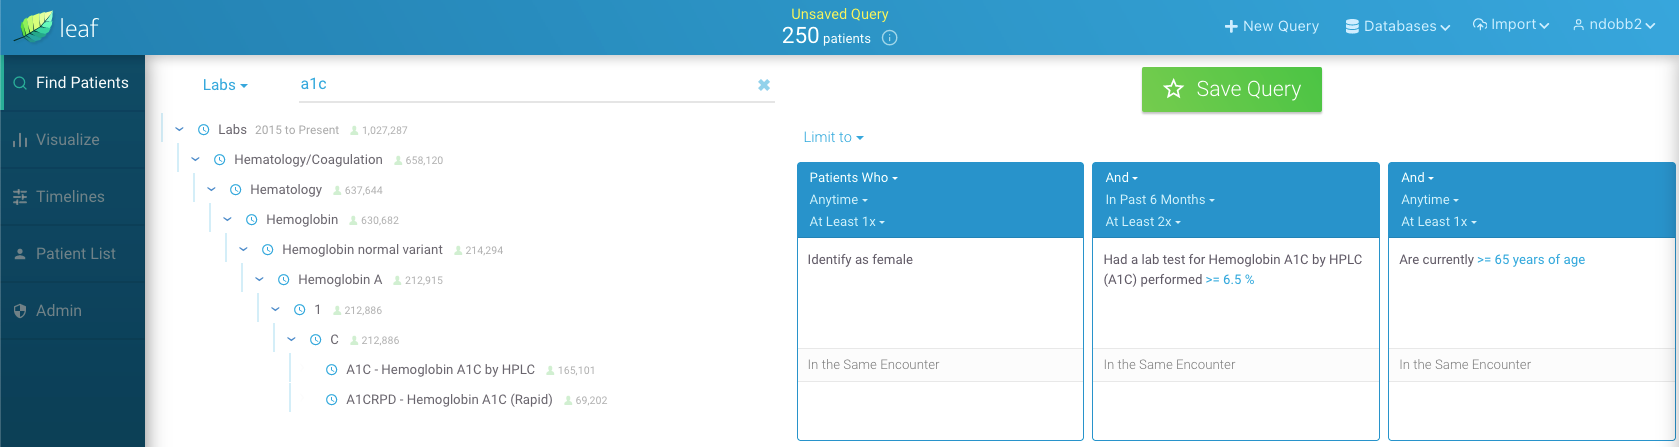
\includegraphics[scale=0.28]{Figures/2_background/leaf_full.png}  
\caption{An example screenshot of the Leaf user interface. The user has generated a query to find patients who identify as female, have had at least two Hemoglobin A1c laboratory results greater than or equal to 6.5 in the past 6 months, and are 65 years of age or older.}
\label{fig_leaf}
\end{figure}

Thus though the aim of this project is to produce an application capable of general purpose cohort discovery - rather than solely for the purposes of clinical trial recruitment - clinical trials are a meaningful and valuable means by which to \textbf{gather data}, \textbf{evaluate performance}, and \textbf{measure potential real-world impact} of solutions for cohort discovery. Moreover, screening software and NLP have been demonstrated to dramatically improve trial recruitment efficiency in many scenarios.
In terms of data, the website \url{https://clinicaltrials.gov}, maintained by the United States National Library of Medicine, hosts freely accessible descriptions of hundreds of thousands of clinical trials from around the world. Because clinical trials enrollments are in many cases recorded in EHRs (which also include the same patients' clinical data), they also can serve as a uniquely objective means of measuring the effectiveness of NLP systems in matching actual enrolled participants based on eligibility criteria. Put another way, an NLP-based system for matching patients to real-world eligibility criteria should reasonably be expected to find many or most patients enrolled in a given clinical trial - with the assumption that patients enrolled in those trials correctly met the necessary criteria as determined by study investigators. Thus however imperfect (e.g., a lack of diagnosis data for an existing condition may cause certain patients to be inappropriately deemed ineligible), clinical trials are thus well-suited for evaluation of NLP-based cohort discovery systems and thus a focus of much of this project.

\section{Challenges in Electronic Screening and NLP in Clinical Trials}

Using NLP to determine patients potentially eligible for a clinical trial has numerous challenges. Consider, for example, a list of eligibility criteria such as\footnote{Adapted from  \url{https://clinicaltrials.gov/ct2/show/NCT03254875}}:

\begin{enumerate}
    \itemsep0em 
    \item \textit{Newly diagnosed with breast cancer and scheduled for surgery}
    \item \textit{18 years or above}
    \item \textit{Those who experience high psychological stress will enter the RCT whereas those with low stress will be followed in an observational questionnaire study}
    \item \textit{No severe psychiatric disease requiring treatment, e.g., schizophrenia}
\end{enumerate}

\noindent While perhaps appearing deceptively simple, this example demonstrates many of the difficulties of this task. In criterion 1,  "Newly" in "Newly diagnosed with breast cancer", suggests that diagnoses occurring further in the past (though how far is unclear) should not be included. Meanwhile, "surgery" in "scheduled for surgery" likely refers to surgery in relation to breast cancer, though this is not explicitly stated. In criterion 2, "18 years" likely refers to participants' age, but this too is not explicitly stated. Criterion 3, meanwhile, is a description of processes which will take place during the trial, but is not actually an eligibility criterion (i.e., participants may be eligible whether their actual stress levels are high or low). In criterion 4, "psychiatric disease" is non-specific and may refer to a large number of unstated conditions, aside from schizophrenia which is given as an example.

Appropriately interpreting the semantics and unstated requirements of these criteria are challenging for NLP systems. For example, an NLP system may correctly determine that "breast cancer" refers to a condition and "surgery" refers to a procedure, but may still fail if "Newly" is not determined to refer to breast cancer or to mean something occurring for the first time. In a subsequent step, an NLP system may normalize (i.e., determine a coded representation of a concept, for example a Unified Medical Language System [UMLS] code) "breast cancer" incorrectly as "Malignant Neoplasms" (C0006826) rather than "Malignant neoplasm of breast" (C0006142). In criterion 3, an NLP system may attempt to limit eligibility to patients with high stress levels, despite the criterion not being a formal restriction as such. In criterion 4, an NLP system may fail to reason that other unstated conditions, such as hysteria or hallucinations, should also be excluded.

Beyond challenges in interpreting eligibility criteria, certain criteria may simply be absent or even incorrect in the data source the NLP system generates a query for. For example, Eastern Cooperative Oncology (ECOG) performance status scores \cite{sok2019objective} are frequently listed in eligibility criteria but often absent in structured clinical databases.

Last, an NLP system capable of identifying patients eligible for clinical trials should also be able to explain \textit{why} patients are eligible and \textit{what it did} to determine eligibility. This step is key to gaining user trust in the system \cite{lundberg2018explainable, jermutus2022influences}, but also challenging as many systems tend to prioritize performance over interpretability.

\section{NLP Methods for Clinical Trial Recruitment}

Various methods for matching eligibility criteria to cohorts of patients using NLP have been put forth by the research community \cite{yuan2019criteria2query, soni2020patient, fang2022combining, zhang2020deepenroll, chen2019clinical, patrao2015recruit, dhayne2021emr2vec, liu2021evaluating, xiong2019cohort}. NLP-based cohort discovery methods hold unique potential and appeal, as they are theoretically able to leverage existing eligibility criteria described in natural language, a medium researchers and investigators already use and are comfortable with. Recent methods which utilize NLP in some form can generally be grouped into 5 categories:

\begin{enumerate}
    \item{\textbf{Database query generation} to Structured Query Language (SQL) or similar systems using either (a) rules, (b) neural network-based encoder-decoder architectures}, or both.
    \item{\textbf{Document ranking and classification} using clinical notes in terms of relevancy vis-à-vis a given eligibility criteria.}
    \item{\textbf{Projection into embeddings} of patient medical history and trial eligibility criteria in a shared vector space and matching via similarity measurement or entailment.}
    \item{\textbf{Logical representations and reasoning} to represent eligibility criteria and patient records, matching by combinations of Semantic Web technologies, ontologies, Description Logics, and rule-based reasoning.}
    \item{A combination of the above.}
\end{enumerate}

\textbf{Database query generation} - SQL-based relational databases are widely used both commercially and within academic institutions, and as such SQL is perhaps unsurprisingly often the target language in natural language to database query research \cite{dar2019frameworks}. Yuan \textit{et al} developed Criteria2Query (shown in Figure \ref{fig_criteria2query}), a hybrid information extraction (IE) pipeline and application which uses both rules and machine learning to generate database queries on an Observational Medical Outcomes (OMOP) \cite{hripcsak2015observational} database. This work was expanded by Fang \textit{et al}, who added functionality for iterative query generation via human correction and adjustment \cite{fang2022combining}. Although not specific to RCTs, other highly relevant recent work on query generation in the biomedical domain has been done using Encoder-Decoder neural architectures for transforming clinical natural language questions into SQL queries \cite{bae2021question, park2021knowledge, wang2020text, pan2021bert, dhayne2021emr2vec}. Park \textit{et al} \cite{park2021knowledge} experimented with transforming medical questions generated in the MIMICSQL data set \cite{johnson2016mimic, wang2020text} using both SQL and SPARQL queries with varying database schema representations. Bae \textit{et al} similarly experimented with methods for handling typos, misspellings, and abbreviations in generating SQL queries from natural language questions. Pan \textit{et al} \cite{pan2021bert} leveraged intermediate abstract syntax tree-based representations and a SQL grammar-based Decoder architecture for dynamic database schema matching. 

\begin{figure}[!ht]
  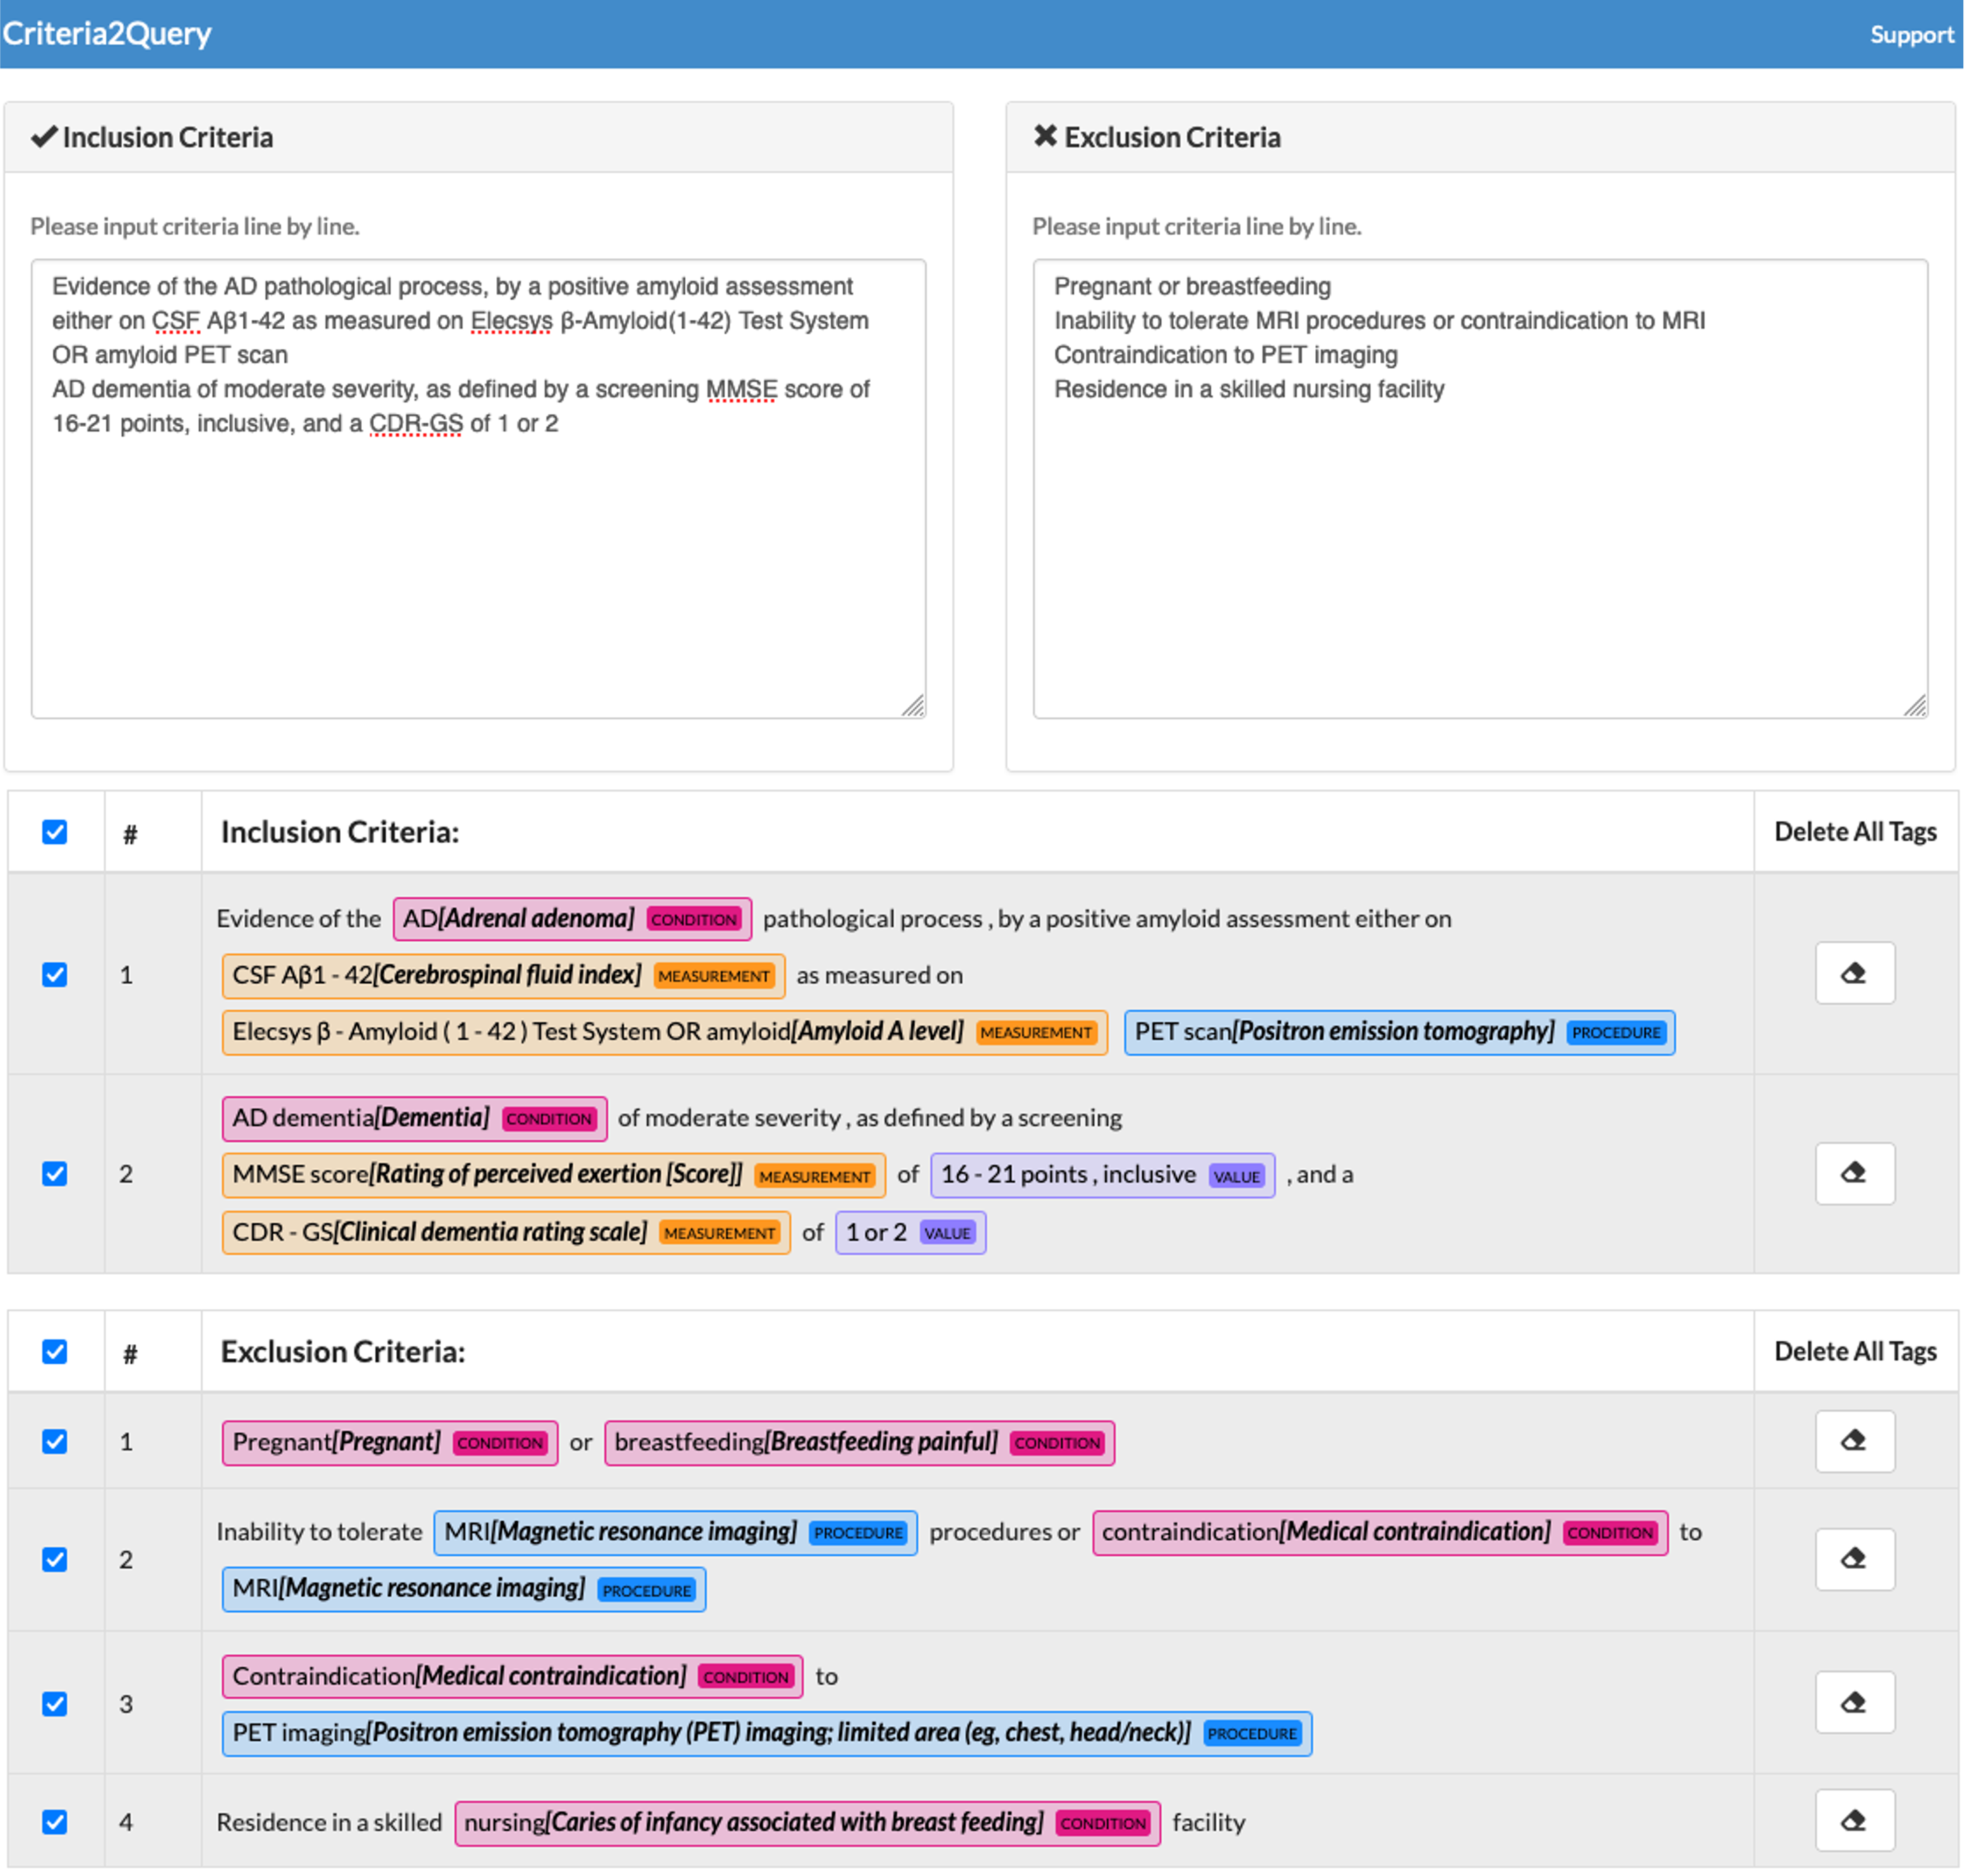
\includegraphics[scale=0.77]{Figures/2_background/criteria2query.png}  
\caption{An example screenshot of the Criteria2Query application. Users type eligibility criteria in free text or enter a clinical trials "NCT" identifier. The application then generates a SQL query and executes it against an OMOP database in order to identify eligible patients.}
\label{fig_criteria2query}
\end{figure}

\textbf{Document ranking and classification} - Focusing on clinical notes, Chen \textit{et al} \cite{chen2019clinical} used hybrid rule-based heuristics and sentence pattern-matching to detect criteria structure, as well as a combination of neural network-based bi-directional long short-term and conditional random field (biLSTM+CRF) architecture and knowledge graphs using the UMLS for determining condition, lab, procedure and drug relationships. Soni and Roberts \cite{soni2020patient} utilized the BERT Transformer architecture \cite{devlin2018bert} and Lucene \cite{lucene} to summarize, rank and classify clinical notes as relevant to a given eligibility criterion, with the most relevant notes predicted to be eligible. 

\textbf{Embedding projections} - Dhayne \textit{et al} \cite{dhayne2021emr2vec} experimented with treating patient-to-RCT matching as a joint embedding and similarity measurement problem while also incorporating the SNOMED-CT ontology to infer basic "is-a" and "has-type" relations between concepts. Similarly, Zhang \textit{et al} \cite{zhang2020deepenroll} used joint patient and eligibility criteria embeddings for entailment prediction, where predicting that a patient can be inferred from a given eligibility criteria equates to eligibility. 

\textbf{Logical representations and reasoning} - Patrao \textit{et al} developed Recruit \cite{patrao2015recruit}, an ontology-driven trial recruitment system which transformed SQL relational data to Resource Description Framework (RDF) graph-based triples. The RDF triples in turn were made query-able by use of an OWL-based reasoning system \cite{owl} and normalization techniques to infer cancer staging. Building upon earlier work \cite{patel2007matching, tu2009ergo, huang2013semanticct}, Baader \textit{et al} \cite{baader2018patient} explored the use of Description Logics and ontologies in matching patients in the MIMIC data set to logical representations of eligibility criteria, for example representing "Diabetes mellitus type 1" as "$\exists_y$.diagnosed\_with(x, y) $\wedge$ Diabetes\_mellitus\_type\_1(y)". Liu \textit{et al} \cite{liu2021evaluating} used domain experts to manually translate criteria into a custom syntax parsable by software. For example, the criterion "Patients more than 18 years old when they received the treatment" would be represented as "$\#Inclusion features['StartDate'] >= demographics['BirthDate'] + @YEARS(18)$". Parsed eligibility criteria were then executed on a proprietary database schema to determine eligible patients.

\section{Corpora}

A key element for any NLP-based approach in identifying patients is robust corpora which capture eligibility criteria semantics sufficiently for high-accuracy query generation. Such corpora can serve as reliable benchmarks for purposes of comparing NLP methods as well as training data sets. A number of corpora have been published. Weng \textit{et al} created EliXR \cite{weng2011elixr}, a pipeline of rule-based methods for syntactic parsing of eligibility criteria using pattern matching. EliXR was validated using a subset of 1,000 randomly selected eligibility criteria annotated by human annotators and compared to syntax trees extracted by their system. This work was expanded by Boland \textit{et al} to support normalization of complex temporal patterns \cite{boland2012elixrtime}. Neither data set was publicly released. Kang \textit{et al} developed EliIE \cite{kang2017eliie}, a hybrid machine-learning and rule-based system for eligibility criteria extraction and normalization. EliIE was evaluated against a human-annotated corpus of eligibility criteria from 230 trials related to Alzheimer's Disease. EliIE was the first system for eligibility criteria extraction which used machine-learning methods (a Conditional Random Field, or CRF \cite{sutton2012introduction}) and the first to use an extraction schema based on the Observational Medical Outcomes Partnership (OMOP) \cite{hripcsak2015observational} common data model. The EliIE corpus was similarly not publicly released, and also limited in terms of generalizability by focusing on Alzheimer's Disease alone. 

More recently, Kury \textit{et al} released Chia \cite{kury2020chia}, a human-annotated corpus of eligibility criteria from 1,000 Phase IV clinical trials across various disease domains. Like EliIE, Chia used an annotation schema based on the OMOP common data model. Following Chia, Sun \textit{et al} created a corpus of COVID-19-related trials' eligibility criteria \cite{sun2021building}. The authors used a similar annotation schema to that of Chia, but included separate annotation layers for cohorts, criterion, named entities, and concepts, which they referred to as a hierarchical annotation model. 

Yu \textit{et al} \cite{yu2020} released a corpus designed for direct text-to-query generation with semantic parsing, however given the relative simplicity of generated queries to date compared to the complexity of clinical databases, it's not clear this approach is yet viable for real-world clinical trials recruitment.

\section{Clinical Knowledge Bases}

A system capable of reasoning on non-specific eligibility criteria necessarily must store some representation of clinical phenomena and their relations. Such information is often described as a knowledge base (KB) \cite{guarino1995ontologies}, or an information store often composed of questions and answers, entities and relations, or factoids. Large-scale KBs, such as DBpedia \cite{lehmann2015dbpedia} are represented as graphs of tuples, where a tuple represents two entities and a relation between them (also often called nodes and edges), such as \{ "asthma", "is-a", "disorder of the respiratory system" \}. Chains of tuple-based entities joined by relations can therefore represent fairly complex phenomena in a compositional fashion. In medicine, the most widely used KB is the Unified Medical Language System, or UMLS \cite{bodenreider2004unified}. The UMLS is a metathesaurus of controlled vocabularies and terminologies such as ICD-9, ICD-10, LOINC, SNOMED, CPT, and others, with mappings between them. While often accessed as a relational database, the UMLS can also be transformed and represented tuple form \cite{noy2009bioportal}. 

Within the clinical domain, KBs (often including the UMLS) have been used for various purposes related to retrieval, reasoning, disambiguation, and question answering. For example, Martinez \textit{et al} and Sankhavara \textit{et al} demonstrated use of the UMLS for query expansion, enabling patient record retrieval via use of synonyms \cite{martinez2014improving, sankhavara2020query}. For reasoning, Shulz and Hahn demonstrated a technique for leveraging the UMLS to reasoning upon anatomical structure \cite{schulz2001medical}. Kazi \textit{et al} demonstrated the use of the UMLS for basic question-answering of medical students \cite{kazi2012medchatbot}. 

More recent work has explored alternative representations of KBs within neural networks. Lin \textit{et al} explored neural network-based inference techniques for inferring missing relations among entities based on other information present in the UMLS and other KBs \cite{lin2018multi}. Hao \textit{et al} and Huang \textit{et al} examined approaches for integrating the UMLS into pre-training of BERT \cite{devlin2018bert} embeddings \cite{hao2020enhancing, huang2020biomedical}. Petroni \textit{et al} point out that even without fine-tuning for a specific domain or task, pre-training of language models with vast data from the internet exhibit reasonable performance on many tasks which necessitate basic reasoning \cite{petroni2019language}.

\section{Summary}

This chapter discussed the importance of clinical trials to biomedical research and human health, as well as challenges in cost and recruitment. We next discussed motivation for and challenges in the use of NLP in patient matching for clinical trials, as well as related research in clinical KBs and published corpora related to clinical trials.

\end{document}